%
\documentclass[a4paper,journal,11pt]{IEEEtran}
\usepackage{blindtext}
\usepackage{vntex}
%\usepackage[utf8]{vietnam}
\usepackage{graphicx}
\usepackage{amsmath,amssymb}
\usepackage{wrapfig}
\usepackage{fancyhdr}
\usepackage{caption}
\usepackage{lipsum}
\usepackage{xcolor}
\usepackage{cite}
\usepackage{listings}
\usepackage{scrextend}
\usepackage{ltxtable}
\usepackage{slashbox}
\usepackage{diagbox}
\usepackage{adjustbox}
\usepackage{multirow}
\usepackage{times}

\renewcommand{\thetable}{\arabic{table}}
%\captionsetup[table]{labelfont=bf, labelsep=period}
%\usepackage[a4paper, total={16cm, 23cm}]{geometry}
\usepackage[left=3.5cm,right=2cm,top=2cm,bottom=2cm]{geometry}
% sd cho harvar
%\usepackage{natbib}
%\usepackage{hyperref}
%
%\fontsize{12pt}{14pt}\selectfont dinh size chu
%
%\author{Nguyễn Văn A$^1$ (tác giả chính), Nguyễn Văn B$^2$ (đồng tác giả),….  % <-this % stops a space
%\thanks{$^{1}$Trường Đại học Trà Vinh}%
%\thanks{$^{2}$Trường Đại học Trà Vinh}%
%\thanks{\hspace{0.1cm} Email:...............................}%
%\thanks{\hspace{0.2cm}Ngày nhận bài: …….. , ngày nhận kết quả bình duyệt: …….., ngày chấp nhận đăng:……….}% <-this % stops a space
%}

% note the % following the last \IEEEmembership and also \thanks - 

 \title{\Large\bf
\changefontsizes{16pt}TIÊU ĐỀ TIẾNG VIỆT
\normalfont
\\
\Large \changefontsizes{14pt} \textit{\\*TIÊU ĐỀ TIẾNG ANH}
}

\begin{document}

\pagestyle{fancy}
\fancyhf{}
\rhead{\changefontsizes{7pt}LĨNH VỰC NGHIÊN CỨU}
\lhead{\changefontsizes{7pt}TẠP CHÍ KHOA HỌC TRƯỜNG ĐẠI HỌC TRÀ VINH, SỐ..., THÁNG ... NĂM ...}
\cfoot{\thepage}
% danh so trang
\pagenumbering{arabic}
%\setcounter{page}{51}
%\cfoot{\leftmark}
% The paper headers
\markboth{TẠP CHÍ KHOA HỌC TRƯỜNG ĐẠI HỌC TRÀ VINH, SỐ..., THÁNG ... NĂM ...}{}
%make the title area
%xoa danh so trang
%\pagenumbering{gobble}
\maketitle
\renewcommand\headrule{}

%\boldmath
%%%%%%%%%%%%%%%%%%%%%%%%%%%%%%%%%%%%%%%%%%%%%%%%%%%%%%%%%%%%%%%%
\textbf{Tóm tắt} -- \textit {Bài báo được đăng trên Tạp chí Khoa học của Đại học Trà Vinh bắt buộc phải mô tả TÓM TẮT nội dung TIẾNG VIỆT của bài báo TẠI ĐÂY}
	
\textbf{\textit {Từ khóa: chèn từ khóa tiếng việt.}}\\
%%%%%%%%%%%%%%%%%%%%%%%%% 

\textbf{Abstract} -- \textit {Bài báo được đăng trên Tạp chí Khoa học của Đại học Trà Vinh bắt buộc phải mô tả TÓM TẮT nội dung TIẾNG ANH của bài báo TẠI ĐÂY}
	
\textbf{\textit {Keywords: chèn từ khóa tiếng anh.}}
\section{GIỚI THIỆU}
	tin giới thiệu được thiết kế để hỗ trợ cho tác giả chuẩn bị bài báo để được xuất bản trên \textsc{TẠP CHÍ KHOA HỌC TRƯỜNG ĐẠI HỌC TRÀ VINH} phiên bản \LaTeX\ 1.0 dùng tập tin TVU.cls (tập tin này được xây dựng tham khảo từ IEEETran.cls).
Với hy vọng giúp tác giả định dạng bài báo khoa học của mình được thuận lợi nhất. \\
Để bắt đầu việc định dạng, tác giả nên tạo một thư mục với tên của bài báo (Ví Dụ như "HuongDan") để chứa tất cả các tập tin (files) liên quan đến bài báo (Ví dụ như: tập tin lớp LATEX - TVU.cls, các hình ảnh, và đồ thì, ...)
%%%%%%%%%%%%%%%%%%%%%%%%%%%%%%%%%%%%%%%%%%%%
\section{MỘT SỐ VẤN ĐỀ LIÊN QUAN}
\subsection{Tiểu tựa}
Nội dung thuộc tiểu tựa có thể biên soạn tại Đây.
	\subsubsection{Tiểu tiểu tựa}
		Nội dung tiểu tiểu tựa
	\subsubsection{Tiểu Tiểu Tựa}
		Nội dung tiểu tiểu tựa
\subsection{Nội dung tiếp theo}
	Tài liệu tham khảo trong đoạn chỉ nêu tài liệu được trích trong báo báo bằng lệnh \cite{tinh}.
	\subsubsection{Trích dẫn tài liệu tham khảo}
	Khi sử dụng cần truy xuất lệnh "\textbackslash cite\{abc\}": tên do người dùng đặt.
	\subsubsection{Trích dẫn hình}
	Khi sử dụng cần truy xuất lệnh "\textbackslash ref\{refhinh1\}": tên do người dùng đặt.
	\subsubsection{Trích dẫn bảng}
	Khi sử dụng cần truy xuất lệnh "\textbackslash ref\{table1\}": tên do người dùng đặt.
\section{GIẢI PHÁP ĐỀ XUẤT}
\subsection{Hình ảnh và bảng biểu}
\subsubsection{Hình ảnh} là phẩn quan trọng, vì vậy những hình ảnh và đồ thị với độ phân giải tốt như yêu cầu từ Tạp chí.

Xin tác giả vui lòng kiểm tra lại các đoạn thẳng và hình vẽ để đảm bảo rằng độ rộng của các đoạn thẳng có thể xem được và theo "Font: time new roman", cũng như các hình ảnh có thể thấy được và không trùng lên nhau. \cite{thuan}

Hình ảnh phải được rõ nét, không bị mờ, xem Hình \ref{fig0} như một ví dụ để tham khảo.

Chú ý:

- Phần "tên file" là tên của tập tin hình.

- Định dạng: PNG, JPG, EPS,...

- Phần "Caption" là nội dung hình muốn hiển thị.
%THÊM HÌNH 1 VÀO BÀI BÁO
\begin{figure}[htp]
\begin{center}
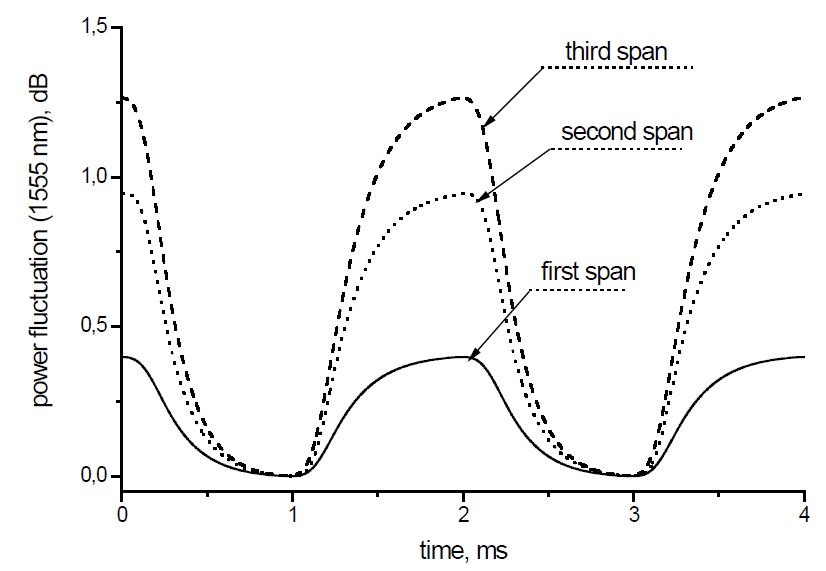
\includegraphics[width=7cm]{f0}
\caption{Ví dụ về độ phân giải của hình ảnh}
\label{fig0}
\end{center}
\end{figure}
\subsubsection{Bảng biểu}Để thêm bảng biểu vào bài báo, tác giả thực hiện với đoạn mã vào vị trí tương ứng trong bài.

Chú ý: Phần "Caption" là nội dung bảng muốn hiển thị. \cite{cuong}

\subsubsection{Công thức} Quy định công thức được trình bày chính giữa cột và trên một dòng riêng biệt.

- Yêu cầu công thức phải được đánh số để dễ tham chiếu \cite{Alby}
\section{THAM KHẢO CÁC LỆNH}
\subsection{Hình ảnh}

\textbackslash begin\{figure\}[htp]

\textbackslash begin\{center\}

\textbackslash includegraphics[width=7.5cm]\{f1\}

\textbackslash caption\{Đoạn mã Latex về cách thêm bảng biểu vào bài báo.\}

\textbackslash label\{fig1\}

\textbackslash end\{center\}

\textbackslash end\{figure\}
\subsection{Bảng biểu}
\begin{table}[htp]
\renewcommand{\arraystretch}{2}
\caption{Ví dụ tạo bảng trong bài báo}
\label{table_example}
\centering
\begin{tabular}{|>{\centering\arraybackslash}p{1cm}|>{\centering\arraybackslash}p{3cm}|>{\centering\arraybackslash}p{2cm}|}
\hline
STT & Họ Tên & Lớp\\
\hline
1 & Nguyễn Văn A & DA11TT\\
\hline
2 & Nguyễn Thị B & DA12TT\\
\hline
\end{tabular}
\end{table}


\textbackslash begin\{table\}[htp]

\textbackslash renewcommand\{arraystretch\}\{2\}

\textbackslash caption\{Ví dụ tạo bảng trong bài báo\}

\textbackslash label\{example\}

\textbackslash centering

\textbackslash begin\{tabular\}\{| | |\}

\textbackslash hline

STT \& Họ Tên

\textbackslash hline

1 \& Nguyễn Văn A \& DA11TT

\textbackslash hline

2 \& Nguyễn Thị B \& DA12TT

\textbackslash hline

\textbackslash end\{tabular\}

\textbackslash end\{table\}

\subsection{Công thức}
\begin{equation} 
\label{eqn_example}
x = \sum \limits_{i= 0}^{z} 2^{i}Q
\end{equation}

\textbackslash begin\{equation\} 

\textbackslash label\{eqn\_example\}

x = \textbackslash sum \textbackslash limits\_\{i= 0\}\^\ \{z\} 2\^\ \{ i \}Q

\textbackslash end\{equation\}

\section{KẾT LUẬN}
Nội dung của phần kết luận được viết TẠI ĐÂY

%%%%%%%%%%%%%%%%%%%%%%%%%%%%%%%%%%%%%%%%%%%%%%%%%%%
\renewcommand\refname{\changefontsizes{10pt}TÀI LIỆU THAM KHẢO}
\bibliography{mybib}
\bibliographystyle{vancouver}

% that's all folks
\end{document}


